\begin{frame}
\frametitle{Maradék gráf}

\begin{columns}
\begin{column}{0.5\textwidth}
\begin{footnotesize}
\begin{itemize}
\item \only<-4>{Csúcsok száma: $n$}\only<5->{\textcolor{red}{Csúcsok száma: $n\leq{}2k^2$}} (pl. $1000$)
\item \only<-3>{Élek száma: $e$}\only<4->{\textcolor{red}{Élek száma: $e\leq{}k^2$}}
\item Kizárható vendégek száma: $k$ (pl. $10$)
\item Csúcsok fokszáma: $1\leq{}d(v)\leq{}k$
\end{itemize}
\emptyline
Mennyi van hátra?

\begin{itemize}
\uncover<2->{
\item Minden kitiltás $\leq{}k$ konfliktust fog megoldani.
\item Még $k$ kitiltásunk maradt.}
\uncover<3->{\item Összesen $\leq{}k^2$ konfliktust tudunk megoldani.}
\uncover<4->{\item $k^2<e$ élre: nem megoldható, készen vagyunk.}
\uncover<5->{\item Fokszám legalább 1: $n\leq{}2k^2$}
\uncover<6->{\item ${{2k^2}\choose{k}}$, pl. ${{200}\choose{10}} \approx 2.24\cdot10^{16}$.\\
Egy mai szuperszámítógépen már megoldható!}
\end{itemize}
\end{footnotesize}
\end{column}

\begin{column}{0.5\textwidth}
\uncover<5->{
\begin{center}
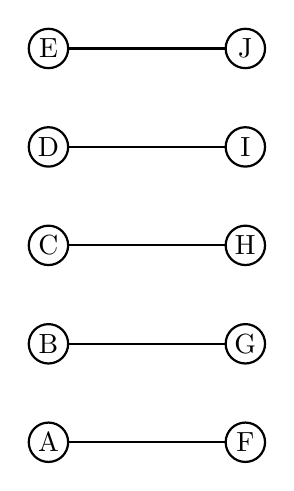
\begin{tikzpicture}[scale=2.5]
\coordinate (A) at (0,0);
\coordinate (B) at (0,0.5);
\coordinate (C) at (0,1);
\coordinate (D) at (0,1.5);
\coordinate (E) at (0,2);
\coordinate (F) at (1,0);
\coordinate (G) at (1,0.5);
\coordinate (H) at (1,1);
\coordinate (I) at (1,1.5);
\coordinate (J) at (1,2);
\draw[thick] (A) -- (F);
\draw[thick] (B) -- (G);
\draw[thick] (C) -- (H);
\draw[thick] (D) -- (I);
\draw[thick] (E) -- (J);
\draw[thick, fill=white] (A) circle (0.1) node {A};
\draw[thick, fill=white] (B) circle (0.1) node {B};
\draw[thick, fill=white] (C) circle (0.1) node {C};
\draw[thick, fill=white] (D) circle (0.1) node {D};
\draw[thick, fill=white] (E) circle (0.1) node {E};
\draw[thick, fill=white] (F) circle (0.1) node {F};
\draw[thick, fill=white] (G) circle (0.1) node {G};
\draw[thick, fill=white] (H) circle (0.1) node {H};
\draw[thick, fill=white] (I) circle (0.1) node {I};
\draw[thick, fill=white] (J) circle (0.1) node {J};
\end{tikzpicture}
\end{center}
}
\end{column}
\end{columns}
\end{frame}
